% !TEX TS-program = pdflatex
% !TEX encoding = UTF-8 Unicode

% This is a simple template for a LaTeX document using the "article" class.
% See "book", "report", "letter" for other types of document.

\documentclass[11pt]{article} % use larger type; default would be 10pt
\usepackage[comma]{natbib}
\usepackage[utf8]{inputenc} % set input encoding (not needed with XeLaTeX)

%%% Examples of Article customizations
% These packages are optional, depending whether you want the features they provide.
% See the LaTeX Companion or other references for full information.

%%% PAGE DIMENSIONS
\usepackage{geometry} % to change the page dimensions
\geometry{a4paper} % or letterpaper (US) or a5paper or....
% \geometry{margin=2in} % for example, change the margins to 2 inches all round
% \geometry{landscape} % set up the page for landscape
%   read geometry.pdf for detailed page layout information

\usepackage{graphicx} % support the \includegraphics command and options

% \usepackage[parfill]{parskip} % Activate to begin paragraphs with an empty line rather than an indent

%%% PACKAGES
\usepackage{amsfonts} % for mathbb
\usepackage{amsmath} % for align
\usepackage{xcolor} % for textcolor
\usepackage{booktabs} % for much better looking tables
\usepackage{array} % for better arrays (eg matrices) in maths
\usepackage{paralist} % very flexible & customisable lists (eg. enumerate/itemize, etc.)
\usepackage{verbatim} % adds environment for commenting out blocks of text & for better verbatim
\usepackage{subfig} % make it possible to include more than one captioned figure/table in a single float
% These packages are all incorporated in the memoir class to one degree or another...
\newtheorem{prop}{Proposition}
\newtheorem{corr}{Corrolary}
%%% HEADERS & FOOTERS
\usepackage{fancyhdr} % This should be set AFTER setting up the page geometry
\pagestyle{fancy} % options: empty , plain , fancy
\renewcommand{\headrulewidth}{0pt} % customise the layout...
\lhead{}\chead{}\rhead{}
\lfoot{}\cfoot{\thepage}\rfoot{}

%%% SECTION TITLE APPEARANCE
\usepackage{sectsty}
\allsectionsfont{\sffamily\mdseries\upshape} % (See the fntguide.pdf for font help)
% (This matches ConTeXt defaults)

%%% ToC (table of contents) APPEARANCE
\usepackage[nottoc,notlof,notlot]{tocbibind} % Put the bibliography in the ToC
\usepackage[titles,subfigure]{tocloft} % Alter the style of the Table of Contents
\renewcommand{\cftsecfont}{\rmfamily\mdseries\upshape}
\renewcommand{\cftsecpagefont}{\rmfamily\mdseries\upshape} % No bold!

% resume enumerate number
\newcounter{break}

%%% END Article customizations

%%% The "real" document content comes below...

\title{Endogenous Grid Method with Two Assets (one illiquid)}
\author{Maximilian Weiß}
\date{October 25, 2022} % Activate to display a given date or no date (if empty),
         % otherwise the current date is printed 

\begin{document}
\maketitle

\section{The story of EGM with two assets (informal)}\label{sec:story}

Consider two households with identical portfolios - owning the same-sized/-quality house, having the same amount of cash - and labor incomes:
the Smiths and the Mullers. We observe them at the beginning of the quarter. Let us assume that we know two values from all households: how much they value owning a little larger house, and how much they value holding a little more cash, at this point in time
(given all the circumstances in the market, like the return on housing and cash, and the business cycle, for instance).
These values are in expectation: since the quarter just began, households do not know yet if and how their labor income changes this quarter,
and whether they will be able to find a trading partner for their house.
While they seem indistinguishable, the two households have different histories: last quarter, the Smiths were active on the housing
market. Meanwhile, the Mullers could not find suitable trading partners for their house, so that they were forced to keep it.

What can we infer about the optimal portfolio choice of households from these data points? First, consider the Mullers.
Last quarter they could not trade their house. However, they can always save more or less in cash. They already had a sense
of how much they would value a little more cash at the beginning of next quarter. Hence, for a given level of their income last quarter, they would
consume more, and hence save less cash, if their value for more cash at the beginning of next quarter was lower, or vice versa.
Since we observe the wealth the Mullers hold now, and can infer if they reduced or increased their cash saving from their valuation
of cash this quarter, we can back out their cash holding from the beginning of last quarter. The only exception to this rule is if the
Mullers faced another constraint last quarter: maybe they would have liked to borrow more than the borrowing limit. Then, the Mullers today
are at the borrowing constraint, and we cannot infer the amount of cash they held last quarter from the consumption level (which is
suboptimal), but instead just note that they follow a ``hand-to-mouth'' rule: they used all cash holdings and (asset and labor) income for consumption. We can furthermore infer that this consumption level must be smaller than if they optimally held debt at the borrowing limit, which implies, for a given asset and labor income-level, a critical value of cash holdings below which they start following the ``hand-to-mouth'' rule.

Next, consider the Smiths. Since they could trade their house last quarter, we know that they likely made a decision to trade off
having more cash or owning a bigger house. They had a sense of how much they would value each of those assets at the beginning of next quarter,
given their portfolio choice. Suppose they now own a big house. We can then infer that their value of having some more cash
is pretty low (maybe they expect higher labor or asset income), or that the house price was particularly low last quarter.
Conversely, if they live in a small house now, their value of having some more cash must be high, or houses were just very expensive
last quarter. If the observed marginal values for cash and housing-wealth (and the house price) do not fit to this optimal trade-off\footnote{More formally, the optimal trade-off prescribes that the (expected) marginal rate of substitution between housing wealth and cash wealth equals the house price. See equation (\ref{eq:pfchoice}) in the formal section below.\label{fn:tradeoff}}
we can infer that the Smiths were financially \textit{constrained} in their choice: they would have liked to short-sell a house (which is not possible), or addtionally to borrow more than the borrowing limit.

In the following, we distinguish the cases when the Smiths were, or were not, financially constrained, and if so, to what extend. First, assume that the Smiths' portfolio fits to the optimal trade-off between cash and houses, as implied by the observed marginal values (see footnote \ref{fn:tradeoff}),
given their income last quarter, and the house price. With respect to their intertemporal decision for cash-holding, we can do the same inference
we applied for the Mullers: If their marginal value for cash was higher today, they would have saved more, and thus consumed less, last quarter.
Following this logic, we can infer the consumption level of the Smiths in the last quarter. However, backing out their cash holding last
quarter is not as easy as with the Mullers, since the Smiths could also finance their consumption and other expenditures by trading houses.
To make progress, we calculate the ``non-human resources'' available to the Smiths last quarter: the sum of the values of their cash, including interest,
and of their house, including rent. This number can be calculated, even though we do not know yet the portfolio of the Smiths last quarter, by
subtracting their labor income last quarter from their consumption and expenditures last quarter. Note that all their expenditures are known, since
we observe their cash and house this quarter, and know the house price from last quarter as well.

The relationship between resources and portfolio choice is monotone: the more resources the Smiths had last quarter, the wealthier they
will be this quarter. Therefore, we can \textit{invert} the relationship: for a given level of resources, we can infer the portfolio that the
Smiths will choose. In fact, this is the best we can do: all (infinitely many) portfolio combinations that yielded the same amount of resources available last quarter, will lead to the same portfolio the Smiths own today.

As a last step, we need to account for the cases were the Smiths were financially constrained last quarter: in that case, while they were able to adjust their housing wealth, the Smiths were constrained by not being able to short-sell a house, or additionally by the borrowing limit on cash. First, we can infer that the Smiths do not own housing-wealth this quarter, because if they did, they would have missed the opportunity to smooth consumption over time: by saving less in housing, which would have cost them rent this quarter, they would have had more money, and thus consumption, last quarter. Let $b^*$ be the amount of cash (for given income last quarter) such that the trade-off between housing wealth (which is zero) and cash is optimal. If the Smiths have less than $b^*$ liquid savings, they were constrained last quarter by not being able to short-sell a house. Then, the Smiths essentially acted like the Mullers: Without regard for the optimal trade-off between cash and housing, they just optimized for the intertemporal cash holding. Hence, their consumption can be backed out from the marginal value of cash today. Thereby, the Smiths' resources can be found. If the Smiths were also borrowing constrained, so that their cash level is at the debt limit today, their consumption is determined by the available resources and labor income, as they followed a ``hand-to-mouth'' rule. Similarly to the case of the binding borrowing constraint for the Mullers, we can infer the critical value of resources below which households start using the ``hand-to-mouth'' rule, by using the optimal consumption level when the Smiths end up at the borrowing limit as an upper bound.

With all these considerations, we are now finally set to ``turn around'' and look forward in time\footnote{Up to this point, we did the ``detective work'' of inferring from observed portfolios of the Mullers and Smiths their wealth last period. Ultimately, however, we are interested in giving forward-looking advice to households. For this purpose, we now compose the information and inferrences collected up to this point into plans of actions.}: From the standpoint of last quarter's portfolio, what would a household with a given labor income and given expected marginal valuations for cash and housing optimally do? First, they take as given exogenously whether they can trade houses during the quarter or not, i.e., whether they are the Smiths or the Mullers. In the case that they are the Mullers, they look if their cash is below a threshold that depends on their labor income and their housing wealth. If that is the case, they borrow up to the debt limit (``hand-to-mouth''-rule). Otherwise, they save as much cash such that their marginal utility from consumption today equals the expected marginal value from having cash next quarter. If they are the Smiths, they first calculate their non-human resources from their cash and housing wealth. If the resources are below a threshold that depends on their labor income, they sell all housing wealth and borrow up to the debt limit (``hand-to-mouth''-rule). If the resources are higher, but below a second threshold that depends on their labor income, they sell all housing wealth, but save an amount of cash that is determined by the expected marginal value of having cash next quarter. Otherwise, they follow the relation between resources and wealth derived above, that maps the level of resources to the optimal housing-cash-combination.

Have we completely described the household problem? Not yet: notice that we took the expected marginal values for cash and housing wealth, depending on this quarter's wealth portfolio and last quarter's labor income, as well as the general economic situation, as given. How do the Smiths and Mullers calculate these values?\footnote{This part corresponds to the formal section (\ref{sec:step2}) below.} For this, we use the trick of recursion: suppose that the Smiths and Mullers have a pretty good guess about these valuations. With them, they make their optimal portfolio choices, and calculate their optimal consumption expenditures for this quarter. Now, they report these optimal consumption levels to a household, say, the Meyers, who today have the exact same portfolio wealth that the Smiths and Mullers entered the quarter with, and the level of labor income that those households had last quarter. The Mullers additionally provide their guess about the marginal value of housing wealth to the Meyers. The Meyers can use the information provided by the Smiths and Mullers to make an even better guess about their expected marginal values for cash and housing wealth: the expected marginal value of cash is given as the weighted average of the marginal utility of consumption of the Smiths and Mullers, where the weight is equal to the probability of being able to be on the housing market during the quarter, multiplied by the gross rate on cash. Calculating the expected marginal value of housing wealth for the Meyers is somewhat more involved: for the case that they will be able to be active on the housing market, they weight the Smiths' marginal utility of consumption with the sum of the price and rent of housing this quarter. For the case that they will not be able to trade their house, they weight the Mullers' marginal utility of consumption with the sum of the house rents this quarter, and the time-discounted guess of the marginal value of housing wealth that the Mullers had.

Finally, the Meyers not only take these informations from the Smiths and Mullers, but also from households that had the same wealth and labor income-history, but experienced a different labor income shock this quarter. Calculating the marginal values as outlined above for these households as well, they construct their final estimate then as the weighted average over all the possible future labor income levels, with the weight equal to their respective probabilities. These probabilities may also depend on the general situation of the economy (the business cycle).

\section{EGM with two assets (formal)}
In the following, I describe in detail the algorithm used in \cite{bayer19}.
\subsection{Preliminaries}
\subsubsection{Household problem}
Let $(b_t^i,d_t^i,z_t^i)$ be the tuple of idiosyncratic states of household $i$, where $b_t^i$ denotes liquid asset holdings (``bonds''), $d_t^i$ denotes illiquid asset holdings (``dividend shares''), and $z_t^i$ denotes idiosyncratic productivity. $b_t^i$ can be negative up to the borrowing limit $\underline{b}$, and $d_t^i$ has to be non-negative. Each period $t$, household $i$ can trade illiquid assets at price $q_t$ with probability $\lambda \in (0,1)$. Idiosyncratic productivity follows a Markov chain with possible values $z_1,..,z_{n_z}$ and the transition matrix $\Pi_z$.

Given their idiosyncratic states, the household has three income sources: labor income, determined by aggregate labor demand and real wages: $z_t^i N_t W_t$; liquid asset income, determined by the net real rate on liquid assets: $(R_t-1)b_t^i$; and illiquid asset income, determined by the dividend: $div_t d_t^i$.

In each period $t$, the household chooses liquid asset holdings $b_{t+1}^i$ and, if possible, illiquid asset holdings $d_{t+1}^i$ in order to maximize their discounted utility stream
\begin{equation}
\sum_{k=0}^{\infty} \beta^k u(c_{t+k}^i),
\end{equation}
subject to the sequence of budget constraints 
\begin{equation}c_{t+k}^i + b_{t+k+1}^i + \mathbb{I}_{\{adj(i,t+k)\}} q_t (d_{t+k+1}^i-d_{t+k}^i) \leq z_{t+k}^i N_{t+k}W_{t+k} + R_{t+k} b_{t+k}^i +  div_{t+k}d_{t+k}^i
\end{equation} for all $k\geq 0$, and the financial constraints $b_{t+1}^i\geq \underline{b}$, $d_{t+1}^i\geq 0$. The indicator variable $\mathbb{I}_{\{adj(i,t)\}}$ equals $1$ iff household $i$ can adjust their illiquid asset holdings in period $t$. $\beta\in (0,1)$ is the time-discount factor and $u(\cdot)$ the period utility function of the household (same across all households). $u(\cdot)$ conforms to the Inada-conditions.
\subsubsection{Value function formalization}
The household problem can be written recursively, defining $V^a_t(b,d|z),V^n_t(b,d|z)$ as the value functions of the household in period $t$ if they can adjust ($V^a_t$) or cannot adjust ($V^n_t$) their illiquid asset holdings. Their recursive definition is as follows:
\begin{align}
V^a_t(b,d|z) &= \max_{b^a\geq\underline{b},\:d^a\geq 0} u(c^a_t(b^a,d^a|b,d,z)) + \beta E_z \left[ \lambda V^a_{t+1}(b^a,d^a|z') + (1-\lambda) V^n_{t+1}(b^a,d^a|z') \right], \\
V^n_t(b,d|z) &= \max_{b^n\geq\underline{b}} u(c^n_t(b^n|b,d,z)) + \beta E_z \left[ \lambda V^a_{t+1}(b^n,d|z') + (1-\lambda) V^n_{t+1}(b^n,d|z') \right],
\end{align}
where $E_z$ denotes the expectation operator conditional on idiosyncratic productivity $z$, and the consumption levels $c^a_t(b^a,d^a|b,d,z)$, $c^n_t(b^n|b,d,z)$ are given by
\begin{align}
c^a_t(b^a,d^a|b,d,z) &= zN_tW_t + R_t b + div_t d - b^a - q_t(d^a-d),\\
c^n_t(b^n|b,d,z) &= zN_tW_t + R_t b + div_t d - b^n.\label{eq:c_n}
\end{align}
\subsubsection{Auxiliary functions}
For the algorithm, it is useful to define the following functions:
\begin{align}
EV_t(b',d'|z) &:= E_z\left[ \lambda V^a_{t+1}(b',d'|z') + (1-\lambda)V^n_{t+1}(b',d'|z') \right], \label{eq:EVdef}\\
\mathcal{R}_t(b,d) &:= R_t b + (div_t+q_t) d.\label{eq:resdef}
\end{align}
The function $EV_t$ can be interpreted as the expected value of the household at the end of period $t$, when the household made their portfolio choice, but the new idiosyncratic productivity has not yet realized and the household does not know yet whether they can trade the illiquid asset next period. The function $\mathcal{R}_t$ maps the portfolio $(b,d)$ into the \textit{non-human resources} available to the household with that portfolio who can adjust their illiquid assets in period $t$.\footnote{$\mathcal{R}_t$ equals cash-at-hand minus labor income, and without accounting for the borrowing limit (since borrowing is an additional resource that households can tap into).}

The first order conditions of the \textit{unconstrained} maximization problem (i.e. abstracting from the lower constraints on $b$, $d^a$) within the value functions are
\begin{align}
- u'(c_t(b',d'|z,\mathcal{R}_t)) + \beta EV_{t,1}(b',d'|z) &\overset{!}{=} 0 \text{ (for }V^a\text{ and }V^n),\label{eq:Euler_b}\\
-q_t u'(c_t(b',d'|z,\mathcal{R}_t)) + \beta EV_{t,2}(b',d'|z) &\overset{!}{=}  0 \text{ (for }V^a), \label{eq:Euler_d}
\end{align}
where the subscripts $1,2$ denote the derivatives by the first and second argument of $EV_t$, and
\begin{equation}
c_t(b',d'|z,\mathcal{R}_t) = z N_t W_t + \mathcal{R}_t - b' - q_t d'. \label{eq:res_cons}
\end{equation}
Note that this parsimonious definition of the consumption level $c_t$ encompasses both the adjustment and non-adjustment case, since in the case of non-adjustment, $d' = d$, so that $\mathcal{R}_t - q d' = R_t b + div_t d$, which shows that equation (\ref{eq:res_cons}) then equals equation (\ref{eq:c_n}).

\subsection{Description of the algorithm}
\textit{Goal}: find optimal portfolio choices and consumption levels in period $t$ for all households on the multi-dimensional wealth and income grid $(b,d,z) \in \{b_1,..,b_{n_b}\} \times \{ d_1,..,d_{n_d} \} \times \{ z_1,..,z_{n_z} \} =: \overline{B} \times \overline{D} \times \overline{Z}$, for both the adjustment and non-adjustment case, i.e. find functions $b^{a,*}_t(b,d,z)$, $d^{a,*}_t(b,d,z)$, $c^{a,*}_t(b,d,z)$ and $b^{n,*}_t(b,d,z)$, $c^{n,*}_t(b,d,z)$.

The algorithm is ``backward-looking'': given the expected future marginal values of the two asset-classes, liquid and illiquid assets, the optimality conditions of the household problem imply the optimal consumption level and asset choices in the present. The method follows the ``endogenous grid''-approach: the variables belonging to the future (here: the expected marginal values of asset holdings) are \textit{on-grid}, while the implied consumption level and asset choices of the present are \textit{off-grid}. To arrive at the optimal policy functions $b^{a,*},d^{a,*},c^{a,*},b^{n,*},c^{n,*}$ as \textit{functions defined on the grid}, the computed optimal choices have to be interpolated over the grid.

While the algorithm shares some parts with the \textit{one-asset} EGM method, the two assets add another important dimension to the household problem: the optimal \textit{portfolio choice} between both assets. Therefore, the algorithm has two main steps. In the first step, the expected marginal values of liquid and illiquid asset holdings, $EV_{t,1}$, $EV_{t,2}$, are taken as given over the grid. This allows to compute the optimal policy functions $b^{a,*}_t$, $b^{n,*}_t$, $d^{a,*}_t$, $c^{a,*}_t$, and $c^{n,*}_t$. This step is comparable to the one-asset EGM method: the marginal value (or, equivalently in the one-asset setting, marginal consumption) of the future implies optimal choices for the present. In the second step, the expected marginal values from last period, $EV_{t-1,1}$ and $EV_{t-1,2}$, are computed using $EV_{t,2}$ and the optimal policy functions. This step is fundamental for the optimal portfolio choice: the household needs to know the different marginal values of both asset classes in order to find the optimal combination of them, in the case where the illiquid asset can be adjusted.

To compute \textit{steady-state} functions  $b^{a,*}$, $b^{n,*}$, $d^{a,*}$, $c^{a,*}$, and $c^{n,*}$, the two steps imply a natural iterative scheme to update $EV_{1}$ and $EV_{2}$ from an initial guess until convergence. To compute \textit{dynamic} paths, $EV_{t,1}$ and $EV_{t,2}$ are part of the state space, and can be solved backward each period with the steps described above.

\textit{Comments about the notation}: Period-subscript $t$ implies that the variable $x_t$ is chosen/defined given all information up to period $t$ (optimal choices depend on information about the aggregate state of the economy). All variables with a \textit{superscript}, may it be ``a'',``*'', or a prime, refer to variables \textit{chosen} that period: either consumption for the contemporaneous period, or assets for the next period. For example, $d^{a,*}_t(b,d,z)$ denotes the level of illiquid assets that the household with idiosyncratic states $(b,d,z)$ will have at the beginning of period $t+1$, and that she chooses in period $t$ (if she can adjust illiquid assets in that period). Conversely, assets \textit{without} a superscript refer to the level of the asset at the beginning of period $t$. In line with the informal story-part (section \ref{sec:story}) and the ``backward-looking'' endogenous grid method, I often refer to choices in period $t$ in the past tense (``last period''), which are inferred from looking at the levels of the variables at the beginning of period $t+1$ (``today''). Whenever a (auxiliary) function is defined \textit{for the first time}, I color it in \textcolor{red}{red}.
\subsubsection{Step 1 (``EGM'')}
\textit{Given}: $EV_{t,1}(b',d'|z)$, $EV_{t,2}(b',d'|z)$ for all $(b',d',z)\in \overline{B} \times \overline{D} \times \overline{Z}$. 
\begin{enumerate}[a.)]
\item First, solve for $b_t^{n,*}$ and $c_t^{n,*}$. This is identical to the EGM-algorithm in the setup with one asset. Take a tuple $(b',d',z)$ on the grid, and assume that the household could not adjust their illiquid asset holdings, so that $d=d'$. First, assume that the household was otherwise financially unconstrained. Then, condition (\ref{eq:Euler_b}) must hold, which gives the optimal consumption level (as a function on grid)
\begin{equation}
u'^{-1}(\beta EV_{t,1}(b',d'|z)) =: \textcolor{red}{c^n_t(b',d'|z)}.\label{eq:Vb2c_n}
\end{equation}
The budget constraint (\ref{eq:c_n}) implies
\begin{align}
&z N_t W_t + R_t b + div_t d' - b' = c^n_t(b',d'|z)\\
\Rightarrow\: & \textcolor{red}{b_t(b',d'|z)} := \frac{c^n_t(b',d'|z)-z N_t W_t -div_t d' + b'}{R_t}
\end{align}
which is the off-grid-\textit{valued} liquid asset holding (defined as function \textit{on} grid) last period.

Second, consider the case where the household was financially constrained. Assume that $b' = \underline{b}$. In the borderline case where this liquid asset choice was optimal, the household consumed $\textcolor{red}{\overline{c}(d'|z)} := c^n_t(\underline{b},d'|z)$\footnote{This is the \textit{upper bound} of consumption in the case that that the household was financially constrained by the borrowing limit.} last period. Solve for last period's liquid asset holding, $b$, as a \textit{function also of last period's consumption}:
\begin{equation}
\textcolor{red}{b_t(b',d,c|z)} := \frac{c + b' - zN_tW_t-div_td}{R_t}.
\end{equation}
Note that this expression does not depend on the Euler equation (\ref{eq:Euler_b}) to hold. If the household was financially constrained by the lower borrowing limit, they consumed less than $\overline{c}(d'|z)$. Hence, they held less liquid assets than $\textcolor{red}{\overline{b}(d'|z)} := b_t(\underline{b},d',\overline{c}(d'|z)|z)$\footnote{In some circumstances, households optimally reduce their liquid savings, $b>\underline{b}$, all the way to the borrowing constraint, $b'=\underline{b}$. $\overline{b}(d'|z)$ denotes the level of savings below which the household does that.}.

Finally, the optimal policy has to be interpolated to the grid $\overline{B}$. The interpolation is usually done linearly: for each tuple $(b,d,z)\in\overline{B}\times\overline{D}\times\overline{Z}$ where $b > \overline{b}$, find the smallest $\hat{b}'\in \overline{B}$ such that $b_t(\hat{b}',d|z)\geq b$, and the largest $\check{b}'\in \overline{B}$ such that $b_t(\check{b}',d|z) \leq b$, and define the interpolated optimal choice $\textcolor{red}{b_t^{n,i}(b,d,z)} := w_b \hat{b}' + (1-w_b) \check{b}'$, where the weights $w_b$ are suitably defined.\footnote{Specifically, the linear weights are given as $w_b = \frac{b-b_t(\check{b}',d,z)}{b_t(\hat{b}',d,z)-b_t(\check{b}',d,z)}$.} The interpolated optimal consumption is analogously given by $\textcolor{red}{c_t^{n,i}(b,d,z)} := w_b c^n_t(\hat{b}',d|z) + (1-w_b) c^n_t(\check{b}',d|z)$\footnote{Note that $d=d'$, so the function defined in (\ref{eq:Vb2c_n}) can be used here.}. Then,
\begin{align}
\textcolor{red}{b_t^{n,*}(b,d,z)} &:= \left\{ \begin{array}{ll} b^{n,i}_t(b,d,z) & b > \overline{b}(d|z) \\ \underline{b} & \text{o.w.} \end{array}  \right., \\
\textcolor{red}{c_t^{n,*}(b,d,z)} &:= \left\{ \begin{array}{ll} c^{n,i}_t(b,d,z) & b > \overline{b}(d|z) \\ zN_tW_t + R_tb + div_t d - \underline{b} & \text{o.w.} \end{array}  \right. ,
\end{align}
give the optimal policy functions in the case of non-adjustment of illiquid asset holdings.
\item Next, solve for the optimal portfolio combination $b_t^a(d'|z)$ for the case that the household could adjust their illiquid asset holdings, and was also otherwise financially unconstrained. We use that conditions (\ref{eq:Euler_b}) and (\ref{eq:Euler_d}) have to hold in this case. By inserting one into the other, we obtain the root finding problem with respect to $b'$
\begin{equation}
\textcolor{red}{\rho_t(b'|d',z)} := EV_{t,2}(b',d'|z)/q_t - EV_{t,1}(b',d'|z) \overset{!}{=} 0.\label{eq:pfchoice}
\end{equation}
Since the expected marginal values are only defined on the grid, we need to find an interpolated $b_t^{a,i}(d'|z)$ for all $(d',z) \in \overline{D}\times\overline{Z}$ such that $\rho_t(b_t^{a,i}(d'|z)|d',z)\approx 0$. To do this efficiently, one should use that $\rho_t$ is monotonely increasing in $b'$\footnote{See proposition \ref{prop:rho} for a proof in steady state. For small deviations from steady state, the property will also hold by virtue of the continuity of the problem. The intuition of the property is that the indifference curve that describes the optimal portfolio allocation is convex.}, since this allows to apply methods that search over sorted lists, like the binary search algorithm. For the largest $\check{b}'\in\overline{B}$ such that $\rho_t(\check{b}'|d',z) \leq 0$ and the smallest $\hat{b}'\in\overline{B}$ such that $\rho_t(\hat{b}'|d',z) \geq 0$, the linear interpolant is defined as $\textcolor{red}{b_t^{a,i}(d'|z)} := w_{d',z} \hat{b}' + (1-w_{d',z})\check{b}'$, with $w_{d',z} = -\frac{\rho_t(\check{b}'|d',z)}{\rho_t(\hat{b}'|d',z)-\rho_t(\check{b}'|d',z)}$.
\setcounter{break}{\value{enumi}}
\end{enumerate}

\textit{Next steps}: We solve for the optimal portfolio choice of households, i.e. when both liquid and illiquid assets could be chosen in period $t$. The central insight is that, for given idiosyncratic productivity $z$, the size of chosen \textit{illiquid} asset wealth increases monotonically in the size of available resources today. Liquid wealth is ``factored out'' by finding the liquid wealth amount that fits optimally to a given $d'$, $b^a(d'|z)$, and then inferring the consumption in period $t$ that fits to this liquid asset choice (in the case of financially unconstrained households). This consumption level, conversely, is used to calculate the available resources in period $t$. In order to account for debt and non-negativity limits, we solve for two thresholds of available resources, $\hat{\mathcal{R}}^a(z)$ and $\check{\mathcal{R}}^a(z)$, along the way.

\begin{enumerate}[a.)]
\setcounter{enumi}{\value{break}}
\item When households are financially unconstrained, the Euler equation (\ref{eq:Euler_b}) has to hold. We can use the computed optimal liquid asset choice $b_t^{a,i}(d'|z)$ to back out last period's consumption level of these households, given their choice of illiquid assets and their labor income that period. Since the marginal value $EV_{t,1}$ is only given as a function on the grid, while the \textit{values} of $b_t^{a,i}$ are off the grid, we have to interpolate $EV_{t,1}$. With on-grid values $\hat{b}'>\check{b}'\in\overline{B}$ that mark the smallest interval $\check{b}'<b_t^{a,i}(d'|z)<\hat{b}'$, a linear interpolant is given as $\textcolor{red}{EV^i_{t,1}(d'|z)} := w_{b^a(d'|z)} EV_{t,1}(\hat{b}',d'|z) + (1-w_{b^a(d'|z)})EV_{t,1}(\check{b}',d'|z)$, where weights $w_{b^a(d'|z)}$ are suitably defined.

Now, calculate the consumption of financially unconstrained households as
\begin{equation}
\textcolor{red}{c^a_t(d'|z)} := u'^{-1}(\beta EV^i_{t,1}(d'|z))
\end{equation}
for all $(d',z)\in \overline{D}\times\overline{Z}$. With this and equation (\ref{eq:res_cons}), the non-human resources available to the household can be computed as a function defined on grid:
\begin{equation}
\textcolor{red}{\mathcal{R}^a_t(d'|z)} := c^a_t(d'|z) - zN_tW_t + b_t^{a,i}(d'|z) + q_t d'.
\end{equation}
\item Compute optimal consumption and available resources in period $t$ for households that could adjust their illiquid asset holdings, but were otherwise financially constrained. Note that financially constrained households have to choose $d'=0$.\footnote{If they chose $d'>0$, and are off their Euler equation (\ref{eq:Euler_b}), they could make a marginal improvement by reducing $d'$, which will imply less dividend income and thus lower future consumption, while it frees up resources to increase consumption today.} If households chose liquid asset holdings $b'$ such that $\underline{b} < b'<b^{a,i}_t(0|z)$, they were constrained by $d'\geq 0$\footnote{By assumption, the household cannot short-sell the illiquid asset.}, but not by the debt limit. Hence, the Euler equation (\ref{eq:Euler_b}) holds, and we can find the consumption level from the $c^n_t$-function in section a): $\textcolor{red}{\tilde{c}_t^a(b'|z)} := c^n_t(b',0|z)$. This allows to compute available resources $\textcolor{red}{\tilde{\mathcal{R}}_t^a(b'|z)} := \tilde{c}^a_t(b'|z) - zN_tW_t + b'$, as well as the first upper limit of available resources, $\textcolor{red}{\hat{\mathcal{R}}^a_t(z)} := \tilde{\mathcal{R}}^a_t(b^{a,i}_t(0|z)|z)$.

If households (with $d'=0$) chose liquid assets at the debt limit, $b'=\underline{b}$, their consumption has an upper bound at $\textcolor{red}{\overline{c}^a(z)} := \tilde{c}^a_t(\underline{b}|z)$. In this case, households are thus twice financially constrained. Analogously to the upper limit on liquid asset holdings $\overline{b}$ in section a), this implies a second upper limit of available resources, $\textcolor{red}{\check{\mathcal{R}}^a_t(z)} := \overline{c}^a(z) - zN_tW_t + \underline{b}$. All households with available resources below $\check{\mathcal{R}}^a_t$ consume ``hand-to-mouth'', that is, all cash-at-hand.

\item Finally, solve for $b^{a,*}_t$, $d^{a,*}_t$ and $c^{a,*}_t$. For a given tuple $(b,d,z)\in \overline{B}\times\overline{D}\times\overline{Z}$, calculate available resources $\mathcal{R}_t(b,d)$ by its definition (\ref{eq:resdef}). For tuples with $\mathcal{R}_t(b,d)>\hat{\mathcal{R}}^a_t(z)$, compute the (linearly) interpolated optimal choices
\begin{align}
\textcolor{red}{d_t^{a,i}(b,d,z)} &:= w_{\mathcal{R}(b,d)}\hat{d}' + (1-w_{\mathcal{R}(b,d)})\check{d}',\\
\textcolor{red}{b_t^{a,i}(b,d,z)} &:= w_{\mathcal{R}(b,d)}b_t^{a,i}(\hat{d}'|z) + (1-w_{\mathcal{R}(b,d)})b_t^{a,i}(\check{d}'|z),\\
\textcolor{red}{c_t^{a,i}(b,d,z)} &:= w_{\mathcal{R}(b,d)}c_t^a(\hat{d}'|z) + (1-w_{\mathcal{R}(b,d)})c_t^a(\check{d}'|z),
\end{align}
where the on-grid values $\hat{d}'>\check{d}'\in\overline{D}$ define the smallest interval such that $\mathcal{R}^a_t(\check{d}'|z) < \mathcal{R}_t(b,d) < \mathcal{R}^a_t(\hat{d}'|z)$, and the weights $w_{\mathcal{R}(b,d)}$ are chosen accordingly.

For tuples with $\check{\mathcal{R}}_t^a(z) < \mathcal{R}_t(b,d) < \hat{\mathcal{R}}_t^a(z)$, compute the (linearly) interpolated optimal choices
\begin{align}
\textcolor{red}{\tilde{b}_t^{a,i}(b,d,z)} &:= \tilde{w}_{\mathcal{R}(b,d)}\hat{\tilde{b}}' + (1-\tilde{w}_{\mathcal{R}(b,d)})\check{\tilde{b}}',\\
\textcolor{red}{\tilde{c}_t^{a,i}(b,d,z)} &:= \tilde{w}_{\mathcal{R}(b,d)}\tilde{c}^a_t(\hat{\tilde{b}}'|z) + (1-\tilde{w}_{\mathcal{R}(b,d)})\tilde{c}^a_t(\check{\tilde{b}}'|z),
\end{align}
where the on-grid values $\hat{\tilde{b}}' > \check{\tilde{b}}'\in\overline{B}$ define the smallest interval such that $\tilde{\mathcal{R}}^a_t(\check{\tilde{b}}'|z) < \mathcal{R}_t(b,d) < \tilde{\mathcal{R}}^a_t(\hat{\tilde{b}}'|z)$, and the weights $\tilde{w}_{\mathcal{R}(b,d)}$ are chosen accordingly. Putting everything together, we have
\begin{align}
\textcolor{red}{b_t^{a,*}(b,d,z)} &:= \left\{ \begin{array}{ll} b^{a,i}_t(b,d,z) & \mathcal{R}_t(b,d) \geq \hat{\mathcal{R}}^a_t(z) \\ \tilde{b}^{a,i}_t(b,d,z) &  \check{\mathcal{R}}^a_t(z) < \mathcal{R}_t(b,d) < \hat{\mathcal{R}}^a_t(z) \\ \underline{b} & \text{o.w.} \end{array}  \right., \\
\textcolor{red}{d_t^{a,*}(b,d,z)} &:= \left\{ \begin{array}{ll} d^{a,i}_t(b,d,z) &\mathcal{R}_t(b,d) \geq \hat{\mathcal{R}}^a_t(z) \\ 0 & \text{o.w.} \end{array}  \right., \\
\textcolor{red}{c_t^{a,*}(b,d,z)} &:= \left\{ \begin{array}{ll} c^{a,i}_t(b,d,z) & \mathcal{R}_t(b,d) \geq \hat{\mathcal{R}}^a_t(z) \\ \tilde{c}^{a,i}_t(b,d,z) &  \check{\mathcal{R}}^a_t(z) < \mathcal{R}_t(b,d) < \hat{\mathcal{R}}^a_t(z) \\ \mathcal{R}_t(b,d) + zN_tW_t - \underline{b} & \text{o.w.} \end{array}  \right. 
\end{align}
\end{enumerate}
\begin{figure}
\centering
\caption{No illiquid adjustment (Step 1.a)}
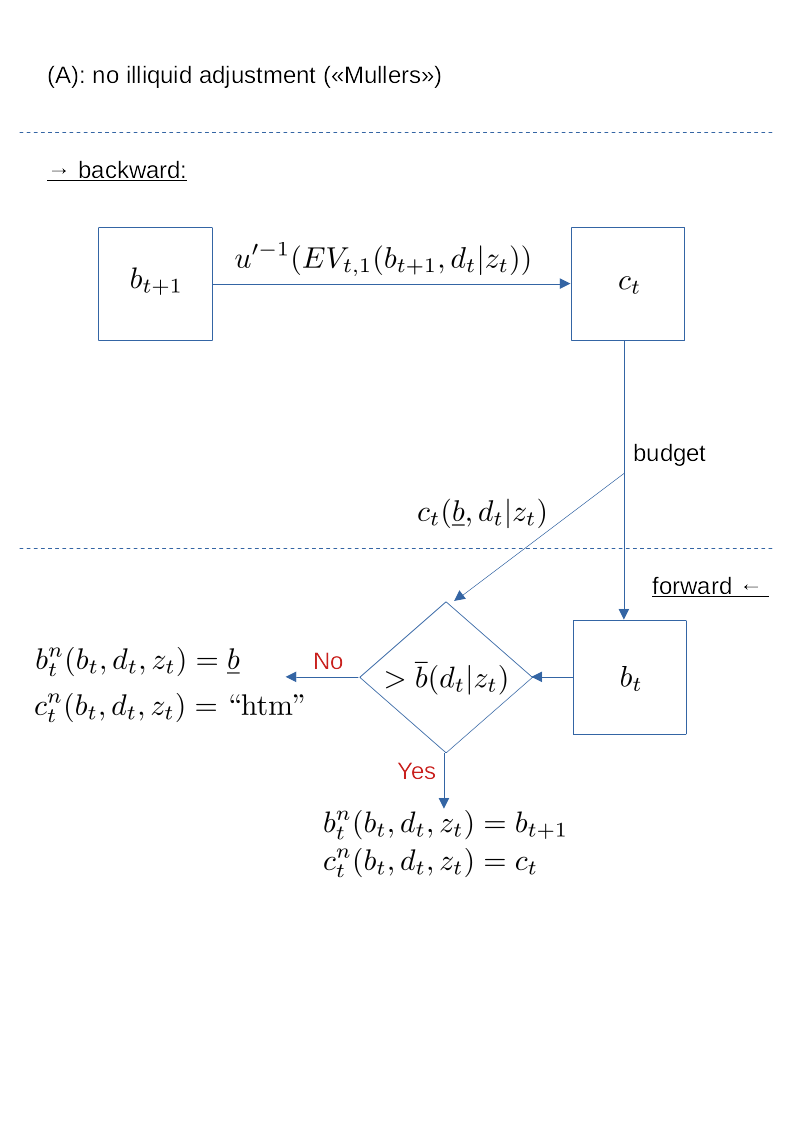
\includegraphics[width=\textwidth]{IllustrationMullers.png}
\end{figure}
\begin{figure}
\centering
\caption{With illiquid adjustment (Steps 1.b-e)}
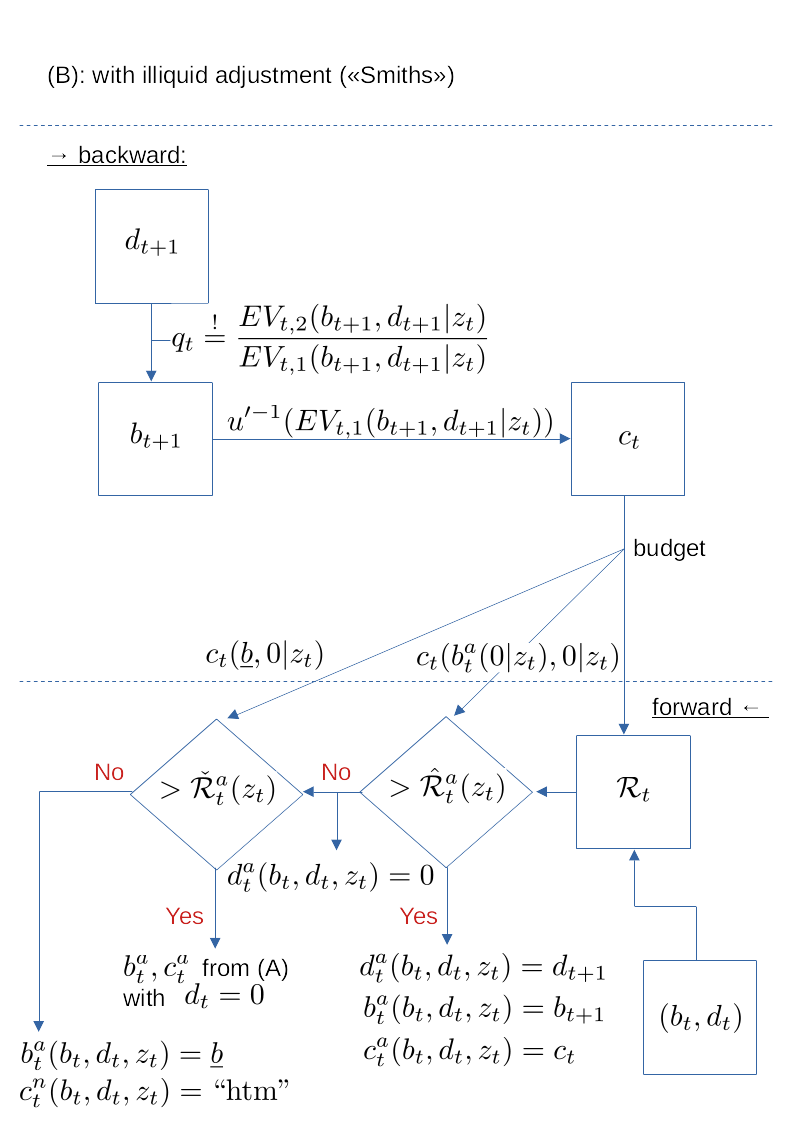
\includegraphics[width=\textwidth]{IllustrationSmiths.png}
\end{figure}
\newpage
\subsubsection{Step 2 (``Update value functions'')} \label{sec:step2}
\textit{Given}: $EV_{t,2}(b,d|z)$, $c_t^{a,*}(b,d,z)$, $c_t^{n,*}(b,d,z)$, $b_t^{n,*}(b,d,z)$ for all $(b,d,z)\in \overline{B}\times\overline{D}\times\overline{Z}$.
\textit{Note}: Since the expected value functions are solved via backward iteration, all asset returns in period $t$ are treated here as deterministic. In general, the expected value function is defined as taking into account also aggregate risk. Therefore, for the general case, one should apply the operator $E_{t-1}$ to the equations below.
\begin{enumerate}[a.)]
\item Compute $EV_{t-1,1}$. By definition (\ref{eq:EVdef}), the derivative of $EV_{t-1}$ by its first argument is
\begin{align}
EV_{t-1,1}(b',d'|z) &= E_{z}\left[ \lambda V^a_{t,1}(b',d'|z') + (1-\lambda) V^n_{t,1}(b',d'|z') \right]\\
& = R_t E_{z}\left[ \lambda u'(c_t^{a,*}(b',d',z')) + (1-\lambda) u'(c_t^{n,*}(b',d',z')) \right],\label{eq:VbMU}
\end{align}
where the second line follows from the envelope theorem:
\begin{equation}
V^{s}_{t,1}(b',d'|z') = \frac{\partial u(c_t^{s,*}(b',d',z'))}{\partial b'} = R_t u'(c_t^{s,*}(b',d',z'))
\end{equation}
for $s=a,n$.
 With idiosyncratic states being the last dimension of the three-dimensional tensor, the expectation over $z'$, given $z$, can be computed for all possible $z_j\in \overline{Z}$ by multiplying the transposed of the transition matrix $\Pi_z$ from the right-hand side:
\begin{equation}
EV_{t-1,1}(b',d'|z_j) = R_t \left[ \lambda u'(c_t^{a,*}(b',d',z')) + (1-\lambda) u'(c_t^{n,*}(b',d',z')) \right]_{z'\in\overline{Z}} \left(\Pi_z^T\right)_{\cdot,j}
\end{equation}
\item Compute $EV_{t-1,2}$.  By definition (\ref{eq:EVdef}),
\begin{align}
EV_{t-1,2}(b',d'|z) &= E_{z}\left[ \lambda V^a_{t,2}(b',d'|z') + (1-\lambda) V^n_{t,2}(b',d'|z') \right]\\
& = E_{z}[ \lambda (q_t+div_t) u'(c_t^{a,*}(b',d',z')) + \label{eq:EVdFull}  \\ & (1-\lambda) ( div_t u'(c_t^{n,*}(b',d',z')) + \beta EV_{t,2}(b_t^{n,*}(b',d',z'),d'|z' )) ] \nonumber,
\end{align}
where the second line follows from applying the envelope theorem (for $V^a$) or just differentiating (for $V^n$):
\begin{align}
V^a_{t,2}(b',d'|z') &= \frac{\partial u(c_t^{a,*}(b',d',z'))}{\partial d'} = (q_t + div_t) u'(c^{a,*}_t(b',d',z')),\\
V^n_{t,2}(b',d'|z') &= \frac{\partial u(c_t^{n,*}(b',d',z'))}{\partial d'} + \beta EV_{t,2}(b^{n,*}_t(b',d',z'),d'|z')\\
&= div_t u'(c^{a,*}_t(b',d',z')) + \beta EV_{t,2}(b^{n,*}_t(b',d',z'),d'|z')
\end{align}
Since the value $b_t^{n,*}(b',d',z')$ is off the grid, we need to interpolate the marginal value of the illiquid asset, such like
\begin{equation}
EV_{t,2}^i(b'',d'|z') = w_{b^{n,*}} EV_{t,2}(\hat{b}'',d'|z') + (1-w_{b^{n,*}}) EV_{t,2}(\check{b}'',d'|z'),
\end{equation}
where $\hat{b}''>\check{b}''\in \overline{B}$ are on grid and determine the smallest interval such that $\check{b}''<b_t^{n,*}(b',d',z')<\hat{b}''$, and the weights $w_{b^{n,*}}$ are chosen accordingly. Rearranging terms and using results from a), $EV_{t-1,2}$ is then computed as
\begin{align}
EV_{t-1,2}(b',d'|z_j)& = div_t E_z[\lambda u'(c^{a,*}_t(b',d',z'))+(1-\lambda)u'(c^{n,*}_t(b',d',z'))] + \nonumber \\
&+ E_z  \left[ \lambda q_t u'(c_t^{a,*}(b',d',z')) + (1-\lambda) \beta EV^i_{t,2}(b'',d'|z') \right] \nonumber\\
&= \frac{div_t}{R_t} EV_{t-1,1}(b',d'|z_j)+\nonumber \\
&+ \left[ \lambda q_t u'(c_t^{a,*}(b',d',z')) + (1-\lambda) \beta EV^i_{t,2}(b'',d'|z') \right]_{z'\in \overline{Z}}\left(\Pi_z^T\right)_{\cdot,j} \label{eq:noarb} 
\end{align}
for all $z_j\in \overline{Z}$.
\end{enumerate}
\textit{Interpretation of equation (\ref{eq:noarb})}: Note that for $\lambda \rightarrow 1$, i.e. the second asset becoming fully liquid, the equation reduces to
\begin{equation}
EV_{t-1,2}(b',d'|z) \overset{(\ref{eq:EVdFull})}{=} (div_t + q_t) E_z u'(c^{a,*}_t(b',d',z')) \overset{(\ref{eq:VbMU})}{=} \frac{div_t+q_t}{R_t} EV_{t-1,1}(b',d'|z),
\end{equation}
which, together with the Euler conditions (\ref{eq:Euler_b}) and (\ref{eq:Euler_d}), and taking expectations, yields the no-arbitrage condition
\begin{equation}
E_{t-1} R_t q_{t-1} u'(c_{t-1}(b,d,z)) = E_{t-1} (div_t+q_t) u'(c_{t-1}(b,d,z)) \Leftrightarrow E_{t-1}\left(R_t -R_t^d\right)=0,
\end{equation}
with $R_t^d := \frac{div_t+q_t}{q_{t-1}}$ as the gross return on illiquid assets. Hence, the ex-ante liquidity premium, $LP_{t-1} := E_{t-1}\left( R_t^d - R_t\right)$, is zero in the case of $\lambda \rightarrow 0$.
\section{Proofs}
\begin{prop}\label{prop:Euler}
In an economy with \textbf{certainty equivalence} with respect to \textbf{aggregate} risk, the ``modified Euler equation''
\begin{equation}
1/R_t^d = \beta E_z \left[ \frac{ u'(c_t^{a,*}(b',d',z'))  - (1-\lambda)\frac{\omega_t}{q_t+div_t}}{u'(c_{t-1}^{a,*}(b,d,z))}\right],\label{eq:modEuler}
\end{equation}
holds, where
\begin{align}
\omega_t := &\omega_t(b',d',z') \nonumber \\:= & (q_t+div_t) u'(c_t^{a,*}(b',d',z'))-(div_t u'(c_t^{n,*}(b',d',z')) +\beta EV_{t,2}(b_t^{n,*}(b',d',z'),d'|z')) \label{eq:wedge}
\end{align}
is the marginal benefit for the household of being able to adjust their illiquid portfolio holdings in period $t$, given their idiosyncratic state $(b',d',z')$\footnote{By the envelope theorem, the marginal value of $d$ when $d'$ can be freely chosen is $(q+div)u'(c^a)$.}.

$(b,d,z)$ is the tuple of idiosyncratic states in period $t-1$, while $(b',d',z')$ is the tuple of idiosyncratic states in period $t$, of a household who is \textbf{financially unconstrained} in period $t-1$.
\end{prop}
\textbf{Proof} I introduce the notation $c_t^{a,*}:=c_t^{a,*}(b',d',z')$, $c_{t-1}^{a,*}:=c_{t-1}^{a,*}(b,d,z)$ and $c_t^{n,*}:=c_t^{n,*}(b',d',z')$ for ease of exposition. Using equation (\ref{eq:noarb}) and taking expectations, and by the definition of $\omega_t$,
\begin{align}
EV_{t-1,2}(b',d'|z) = E_{t-1}\left[ \frac{div_t}{R_t} EV_{t-1,1}(b',d'|z) + q_tu'(c_t^{a,*}) - (1-\lambda)(\omega_t - div_t (u'(c_t^{a,*})-u'(c_t^{n,*})))\right]
\end{align}
Imposing certainty equivalence and rearranging terms yields
\begin{align}
EV_{t-1,2}(b',d'|z) = &\frac{div_t}{R_t} EV_{t-1,1}(b',d'|z) -  div_t E_z\left[(1-\lambda)u'(c_t^{n,*})+\lambda u'(c_t^{a,*}) \right] +\\ & E_z\left[ u'(c_t^{a,*})(q_t + div_t) - (1-\lambda)\omega_t\right]\\
\overset{(\ref{eq:VbMU})}{=} &  E_z\left[ u'(c_t^{a,*})(q_t + div_t) - (1-\lambda)\omega_t\right]
\end{align}
Since the household is financially unconstrained in period $t-1$, they are on the Euler equation for illiquid assets, (\ref{eq:Euler_d}), so that
\begin{align}
q_{t-1} u'(c_{t-1}^{a,*}) &= \beta E_z\left[ u'(c_t^{a,*})(q_t + div_t) - (1-\lambda)\omega_t\right]\\
\Leftrightarrow \frac{q_{t-1}}{q_t+div_t} &= \beta E_z \left[ \frac{u'(c_t^{a,*}) - (1-\lambda)\frac{\omega_t}{q_t+div_t}}{u'(c_{t-1}^{a,*})} \right] 
\end{align}
\begin{corr}\label{corr:LP}
The ex-ante liquidity premium can (under aggregate certainty equivalence) be characterized as
\begin{equation}
\frac{LP_{t-1}}{R_t} = \beta (1-\lambda) \frac{q_t}{q_{t-1}} E_z \left[ \frac{u'(c_t^{n,*}) - \frac{\beta EV_{t,2}(b^{n,*}_t,d'|z')}{q_t}}{u'(c_{t-1}^{a,*})} \right]
\end{equation}
\end{corr}
\textbf{Proof} As another notational shortcut, define $b^{n,*}_t := b^{n,*}_t(b',d',z')$. By assumption, the household with idiosyncratic state $(b,d,z)$ is financially unconstrained, so that they are on the Euler equation with respect to the liquid asset:
\begin{equation}
1/R_t = \beta E_z\left[ \frac{\lambda u'(c^{a,*}_t)+(1-\lambda) u'(c^{n,*}_t)}{u'(c^{a,*}_{t-1})}\right]
\end{equation}
Combining this with the result of proposition \ref{prop:Euler}, I get
\begin{align}
1/R_t - 1/R_t^d = & \beta (1-\lambda) E_z\left[ \frac{\frac{\omega_t}{q_t+div_t}-(u'(c_t^{a,*})-u'(c_t^{n,*}))}{u'(c_{t-1}^{a,*})} \right]\\
\overset{(\ref{eq:wedge})}{=} & \beta (1-\lambda) E_z \left[ \frac{u'(c_t^{a,*}) - \frac{div_t u'(c_t^{n,*}) + \beta EV_{t,2}(b_t^{n,*},d'|z')}{q_t+div_t} - (u'(c_t^{a,*})-u'(c_t^{n,*}))}{u'(c_{t-1}^{a,*})} \right]\\
= & \beta(1-\lambda) E_z\left[ \frac{\frac{q_t}{q_t+div_t}u'(c_t^{n,*})+ \frac{\beta EV_{t,2}(b_t^{n,*},d'|z')}{q_t+div_t}}{u'(c_{t-1}^{a,*})} \right]
\end{align}
Multiplying with $R_t^d$ yields
\begin{align}
R_t^d/R_t - 1 = \beta (1-\lambda) E_z\left[ \frac{\frac{q_t}{q_{t-1}}u'(c_t^{n,*}) +  \frac{\beta EV_{t,2}(b_t^{n,*},d'|z')}{q_{t-1}}}{u'(c_{t-1}^{a,*})}\right]
\end{align}
and thus the claim.
\begin{corr}\label{corr:LPpos}
With illiquid assets, $\lambda<1$, the ex-ante liquidity premium is positive: $LP_{t-1}>0$.
\end{corr}
\textbf{Proof} In expectation, households that cannot adjust their illiquid asset holdings are off their Euler equation with respect to that asset, i.e.
\begin{equation}
E_z \left[ \beta EV_{t,2}(b_t^{n,*}(b',d',z'),d'|z')/q_t - u'(c^{n,*}_t(b',d',z')) \right] <0,
\end{equation}
since the case where $d' = d_t^{a,*}(b',d',z')$ is a zero probability event if the idiosyncratic productivity shocks follow a continuous distribution\footnote{When the distribution is approximated by a finite state-process, the probability is still very small.}. By corrolary \ref{corr:LP}, then, $LP_{t-1}>0$.


\begin{prop}\label{prop:rho}
Assume a calibration where the steady state interest rate on saving is positive, i.e. $R>1$.

Then, in steady state, $\rho(b'|d',z)$, as defined in equation (\ref{eq:pfchoice}), is increasing in $b'$, i.e.
\begin{equation}
\frac{\partial \rho(b'|d',z)}{\partial b'} = \frac{EV_{21}(b',d'|z)}{q} - EV_{11}(b',d'|z) > 0,
\end{equation}
when $(b',d')$ are an optimal choice of a household with idiosyncratic productivity $z$.
\end{prop}
\textbf{Proof} Let $EV_1(b',d'|z),EV_2(b',d'|z)$ denote the expected marginal values of liquid and illiquid assets in steady state, respectively.
%\begin{align}
%\frac{EV_2(b',d'|z)}{q} \overset{(\ref{eq:noarb})}{=} &\frac{div}{Rq} EV_1(b',d'|z) + \\ &E_{z}\left[ \lambda u'(c^{a,*}(b',d',z')) + \beta(1-\lambda)\frac{EV_2(b^{n,*}(b',d',z'),d'|z')}{q} \right]\\
%\overset{(\ref{eq:LPnonadj})}{=} &\frac{div}{Rq} EV_1(b',d'|z) + \\ &E_{z}\left[  \lambda u'(c^{a,*}(b',d',z')) + (1-\lambda) u'(c^{n,*}(b',d',z'))\right] - \frac{LP u'(c^{a,*}(b,d,z))}{R\beta}\\
%= &\frac{R^d}{R}EV_1(b',d'|z)-\frac{LP u'(c^{a,*}(b,d,z))}{R\beta}
%\end{align}
%Subtracting by $EV_1(b',d'|z)$ yields an expression for $\rho$:
%\begin{align}
%\rho(b'|d',z) = \frac{LP}{R}\left( EV_1(b',d'|z) - \frac{u'(c^{a,*}(b,d,z))}{\beta}\right)\label{eq:rho}
%\end{align}
\begin{align}
\rho(b'|d',z) =& \frac{EV_2(b',d'|z)}{q}-EV_1(b',d'|z) \\ \overset{ (\ref{eq:noarb})}{=}& \left( \frac{div}{Rq} - 1 \right) EV_1(b',d'|z) + E_z\left[ \lambda u'(c_1^{a,*}) + \beta (1-\lambda) EV_2(b_1^{n,*},d'|z')\right]\\
\overset{(\ref{eq:wedge})}{=} &  \left( \frac{div}{Rq} - 1 \right) EV_1(b',d'|z) + E_z [ \lambda u'(c_1^{a,*}) +\nonumber \\ & (1-\lambda) (q u'(c_1^{a,*}) - div( u'(c_1^{n,*})-u'(c_1^{a,*}))-\omega) ]\label{eq:rhostep1}
\end{align}
Next, I use proposition \ref{prop:Euler} together with the Euler equation of the liquid asset to derive an expression for $\omega$ that depends only on period 1-optimal choices and aggregate returns. By the Euler equation, it holds that
\begin{align}
u'(c^{a,*}_0) = \beta R E_z [\lambda u'(c^{a,*}_1)+(1-\lambda) u'(c^{n,*}_1)]
\end{align}
By proposition \ref{prop:Euler}, then,
\begin{align}
&1/R^d = \frac{E_z\left[ u'(c^{a,*}_1)-(1-\lambda)\frac{\omega}{q+div}\right] }{RE_z[\lambda u'(c^{a,*}_1)+(1-\lambda)u'(c^{n,*}_1)]}\\
\Leftrightarrow& \frac{R}{R^d}E_z[\lambda u'(c^{a,*}_1)+(1-\lambda) u'(c^{n,*}_1)] - E_z[u'(c_1^{a,*})] = -(1-\lambda)\frac{E_z[\omega]}{q+div}\\
\Leftrightarrow & E_z[u'(c^{a,*}_1)] \left( \lambda \frac{R}{R^d} - 1\right) + E_z[u'(c^{n,*}_1)] (1-\lambda) \frac{R}{R^d} = -(1-\lambda) \frac{E_z[\omega]}{R^d q}\\
\Leftrightarrow &\frac{R^d - \lambda R}{1-\lambda} E_z[u'(c^{a,*}_1)] - R E_z[u'(c^{n,*}_1)]  = \frac{E_z[\omega]}{q}\\
\Leftrightarrow & E_z[\omega] = Rq \left( \frac{R^d/R-\lambda}{1-\lambda} E_z[u'(c^{a,*}_1)]-E_z[u'(c^{n,*}_1)] \right)
\end{align}
Inserting this back into equation (\ref{eq:rhostep1}), using equation (\ref{eq:VbMU}), and collecting terms:
\begin{align}
\rho(b'|d',z)=&\left(\frac{div}{Rq}-1\right) R E_z[\lambda u'(c^{a,*}_1)+(1-\lambda)u'(c^{n,*}_1)] +\nonumber \\
+&  E_z[u'(c^{a,*}_1)](\lambda + (1-\lambda)(q-1)) - (1-\lambda)div E_z[u'(c^{n,*}_1)] -\nonumber \\- &  Rq ( (R^d/R-\lambda) E_z[u'(c^{a,*}_1)] - (1-\lambda) E_z[u'(c^{n,*}_1)])\\
= & E_z[u'(c^{a,*}_1)]\left(\lambda (R^d-1-R+1+Rq)+(1-\lambda)(q-1)-R^dq\right) + \nonumber \\
+& E_z[u'(c^{n,*}_1)](1-\lambda)(R^d-1-R-div+Rq)\\
= & E_z[u'(c^{a,*}_1)] \left( \lambda(LP - qLP) + (1-\lambda)(q-1-qR^d) \right)+\nonumber \\+ &E_z[u'(c^{n,*}_1)](1-\lambda)\left(LP - 1 - q(LP - 1)\right)\\
=& q(1-\lambda) \left\{ E_z[u'(c^{a,*}_1)] (1-R^d) + E_z[u'(c^{n,*}_1)] (1-LP) \right\}- \nonumber \\
-& E_z[u'(c^{a,*}_1)]( 1-\lambda+\lambda(q-1)LP)-E_z[u'(c^{n,*}_1)](1-\lambda)(1-LP)
\end{align}
Using $\frac{\partial u'(c^{a,*}_1)}{\partial b'} = R u''(c^{a,*}_1)$ and $\frac{\partial u'(c^{n,*}_1)}{\partial b'} = R u''(c^{n,*}_1)$, the claim of the proposition holds iff
\begin{align}
&-E_z[u''(c^{a,*}_1)](1+\lambda(LP(q-1)-1)) - E_z[u''(c^{n,*}_1)](1-\lambda)(1-LP)\nonumber \\> &-q(1-\lambda) \left\{  E_z[u''(c^{n,*}_1)] (1-LP) -E_z[u''(c^{a,*}_1)] (R^d-1) \right\}\label{ineq:toshow}
\end{align}

Without loss of generality, normalize the steady state value of the price of capital to 1, i.e. $q=1$. Then, inequality (\ref{ineq:toshow}) simplifies to
\begin{align}
    -(1-\lambda) E_z[u''(c^{a,*}_1)] > (1-\lambda) E_z[u''(c^{a,*}_1)](R^d-1)
\end{align}
Note that $u''(\cdot)<0$ by assumption of a concave utility function. Hence, $E_z[u''(c^{a,*}_1)]<0$, and with $\lambda \in (0,1)$ and positive interest rates (by assumption), implying $R^d>1$ due to $LP>0$ by corollary \ref{corr:LPpos}, the claim follows.
%First, I derive a necessary and sufficient condition for inequality (\ref{ineq:toshow}) to hold for a given, realized productivity level $z'$. Dividing by $-u''(c^{n,*}_1)$ yields
%\begin{align}
%\xi [1+\lambda(LP(q-1)-1)]+(1-\lambda)(1-LP)>q(1-\lambda)[(1-LP)+\xi(R^d-1)],
%\end{align}
%where $\xi := u''(c^{a,*}_1)/u''(c^{n,*}_1)$ is the ratio of curvatures of the utility function at the consumption levels when households can or cannot adjust.
% Multiplying both sides by $R$ yields
%\begin{align}
%R\rho(b'|d',z) = &(LP -1)EV_1(b',d'|z) + E_z[\lambda R u'(c^{a,*})+\\ &(1-\lambda)(\beta R^d EV_1(b^{n,*},d'|z')-LP u'(c^{a,*}))] \\ = & (LP-1)EV_1(b',d'|z) + E_z[(\lambda R^d - LP)u'(c^{a,*})+(1-\lambda) R^d \beta EV_1(b^{n,*},d'|z')]
%\end{align}
%First, assume that $b^{n,*}>\underline{b}$ (or, equivalently, $b' > \overline{b}(d',z')$). Then, Euler equation (\ref{eq:Euler_b}) implies
%\begin{align}
%R\rho(b'|d',z) = & (LP-1)EV_1(b',d'|z) + E_z[R^d(\lambda u'(c^{a,*}) + (1-\lambda)u'(c^{n,*}))-LP u'(c^{a,*})],
%\end{align}
%where $c^{n,*}:= c^{n,*}(b',d',z')$ follows the established notation. Using again optimality condition (\ref{eq:VbMU}), this simplifies to
%\begin{align}
%R \rho(b'|d',z) = &\left(LP - 1 + \frac{R^d}{R} \right) EV_1(b',d'|z) - LP E_z[u'(c^{a,*})]\\
%				= & LP\left( \left( 1 + \frac{1}{R}\right) EV_1(b',d'|z) - E_z[u'(c^{a,*})]\right)
%\end{align}
%Note that this expression of $\rho$ is substantially different from equation (\ref{eq:rho}), since the optimal consumption $c^{a,*} = c^{a,*}(b',d',z')$ is chosen in the period \textit{after} idiosyncratic productivity $z$ was drawn, and depends on saved bonds $b'$ in a straightforward functional way: $\frac{\partial c^{a,*}}{\partial b'} = R$.
%
%To proof the claim in this case, it is to show that
%\begin{equation}
%\left(1+\frac{1}{R}\right) EV_{11}(b',d'|z) - R E_z[u''(c^{a,*})] > 0.\label{eq:ineqrho}
%\end{equation}
%From equation (\ref{eq:VbMU}), it follows that
%\begin{equation}
%EV_{11}(b',d'|z) = RE_z[\lambda u''(c^{a,*}) + (1-\lambda) u''(c^{n,*})]
%\end{equation}
%Inserting this into inequality (\ref{eq:ineqrho}) and rearranging yields
%\begin{align}
%R(1-\lambda) E_z[u''(c^{n,*})-u''(c^{a,*})] > -E_z[\lambda u''(c^{a,*}) + (1-\lambda) u''(c^{n,*})]
%\end{align}
%
%From these arguments, it follows that
%\begin{align}
%\frac{EV_{21}(b^{(1)},d'|z^{(0)})}{q} = & R E_{z^{(0)}} \left[ \lambda R^d u''(c^a_1(b^{(1)})) + (1-\lambda)\frac{div}{q} u''(c^n_1(b^{(1)})) \right],\label{eq:EV21}
%\end{align}
%where the gross return on liquid assets, $R$, is the interior derivative of the consumption levels by the liquid asset holding $b^{(1)}$, and hence is multiplied with the second derivatives of the utility function by virtue of the chain rule.
%
%For the marginal expected value of liquid assets, it holds that
%\begin{equation}
%EV_{11}(b^{(1)},d'|z^{(0)}) \overset{(\ref{eq:VbMU})}{=} R^2 E_{z^{(0)}} \left[ \lambda u''(c^a_1(b^{(1)}))+(1-\lambda)u''(c^n_1(b^{(1)})) \right].\label{eq:EV11}
%\end{equation}
%Subtracting equation (\ref{eq:EV11}) from (\ref{eq:EV21}), we get the derivate of $\rho(b'|d',z)$ by $b'$.\footnote{From now on, $b' = b^{(1)}$ and $z = z^{(0)}$ for better readability.}. We reduce the complexity of the equations with some algebraic steps:
%\begin{align}
%\frac{\partial \rho(b'|d',z)}{\partial b'} &> 0 \\ \Leftrightarrow  E_{z}\left[\lambda R^d u''(c^a_1(b')) + (1-\lambda)\frac{div}{q}u''(c^n_1(b'))\right] &> R E_{z}\left[ \lambda u''(c^a_1(b')) + (1-\lambda) u''(c^n_1(b')) \right]\\
%\Leftrightarrow  \lambda LP E_z [u''(c^a_1(b'))] &> (1-\lambda) (R - \underbrace{\frac{div}{q}}_{R^d-1} ) E_z[u''(c^n_1(b'))]\\
%\Leftrightarrow E_z[u''(c^a_1(b'))] &> \frac{(1-\lambda)(1-LP)}{\lambda LP} E_z[u''(c_1^n(b'))],\label{eq:MUineq}
%\end{align}
%where $LP = R^d-R>0$ is the steady state liquidity premium.
%
%To see that inequality (\ref{eq:MUineq}) holds, first note that
%\begin{equation}
%\frac{(1-\lambda)(1-LP)}{\lambda LP} = \left( 1 + \frac{1-\lambda - LP}{\lambda LP}\right) > 1,
%\end{equation}
%since $LP + \lambda < 1$ for all sensible calibrations (for example, $\lambda = 0.1$ and $LP = 0.02$). By concavity of the utility function, $E_z[u''(c_1^n(b'))]$ is negative. Additionally, if households always consumed more when they can adjust their illiquid asset holdings, $c^a\geq c^n$, the property of \textit{prudence}, $u'''>0$, would yield
%\begin{equation}
%E_z[u''(c_1^a(b'))] > E_z[u''(c_1^n(b'))],
%\end{equation}
%and hence the desired result.
%
%However, it can be the case that $c^a < c^n$. The reason is that, for households who are away from the borrowing constraint, but not yet very wealthy, it can be beneficial to sacrifice some consumption during the adjustment period in order to increase their illiquid wealth holding. 
\bibliographystyle{agsm}
\bibliography{refs}
\end{document}
